\section{Setup description}
In this project we are going to simulate a client and a server using containers to have the possibility to use multiple devices at the same time and to have this project running on other devices keeping all the variables and the development environment without having to re-create them from scratch.

When a user wants to register a new device, they already know the device ID, which is pre-configured. However, there is no direct way to verify the validity of an ID during registration. To prevent malicious users from forging IDs, the protocol denies access if the secure vault isn't already linked to a device ID checking its presence into a server database, ensuring that only legitimate devices can connect. The sensors in this setup are emulated to simulate real-world behavior. On server and client side, Python is used because of its robustness and ability to handle complex logic.\\

\begin{figure}[h]
    \centering
    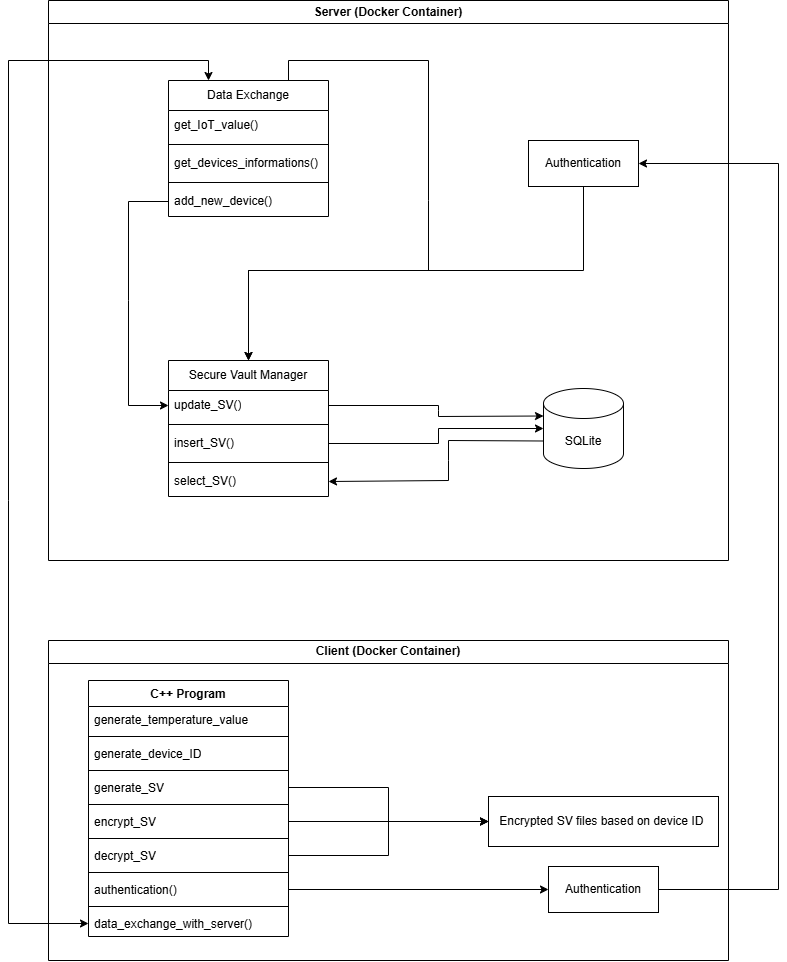
\includegraphics[width=.48\textwidth]{imgs/IoT_auth.png}
    \caption{UML Diagram}
    \label{fig:name}
\end{figure}

The SQLite database is encrypted and only the Secure Vault Manager has the key to read and write from and on it.